% Topic from _Linear Algebra_ Jim Hefferon
%  http://joshua.smcvt.edu/linalg.html
%  2012-Feb-12
\topic{Magic Squares}
\index{magic squares|(}
A Chinese legend tells the story of a  
flood by the Lo river.
The people offered sacrifices to appease the river.
Each time from the river a turtle emerged, 
walked around the sacrifice, and returned to the river.
Fuh-Hi, % (2858-2738~BC)
the founder of Chinese civilization,
interpreted this to mean that
the river did not accepted the sacrifices.  
A child provided the answer by noticing 
that on its shell the turtle had what is today
called the pattern of Lo Shu (``river scroll'').
\begin{center}
  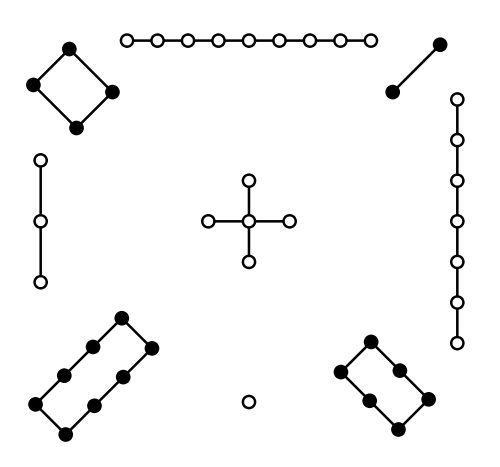
\includegraphics[height=1in]{LoShu.png}
\end{center}
The dots make a matrix.
\begin{center}
  \begin{tabular}{|c|c|c|}
    \hline
      $4$  &$9$  &$2$  \\ \hline
      $3$  &$5$  &$7$  \\ \hline
      $8$  &$1$  &$6$  \\ \hline    
  \end{tabular}
\end{center}
Each row, column, 
and diagonal adds to $15$
(the number of days in each of the twenty four cycles of the 
Chinese solar year).
Now that the people knew how much to sacrifice, at last the river's anger cooled.
% (http://en.wikipedia.org/wiki/Lo_Shu_Square)

A square matrix is 
\definend{magic}\index{magic square}\index{matrix!magic square}
if each row, column, and diagonal add to the same
value, the matrix's \definend{magic number}.

Another example of a magic square appears in the engraving
\textit{Melencolia I} by Albrecht D\"urer.
% (http://en.wikipedia.org/wiki/Melencolia_I)
\begin{center}
  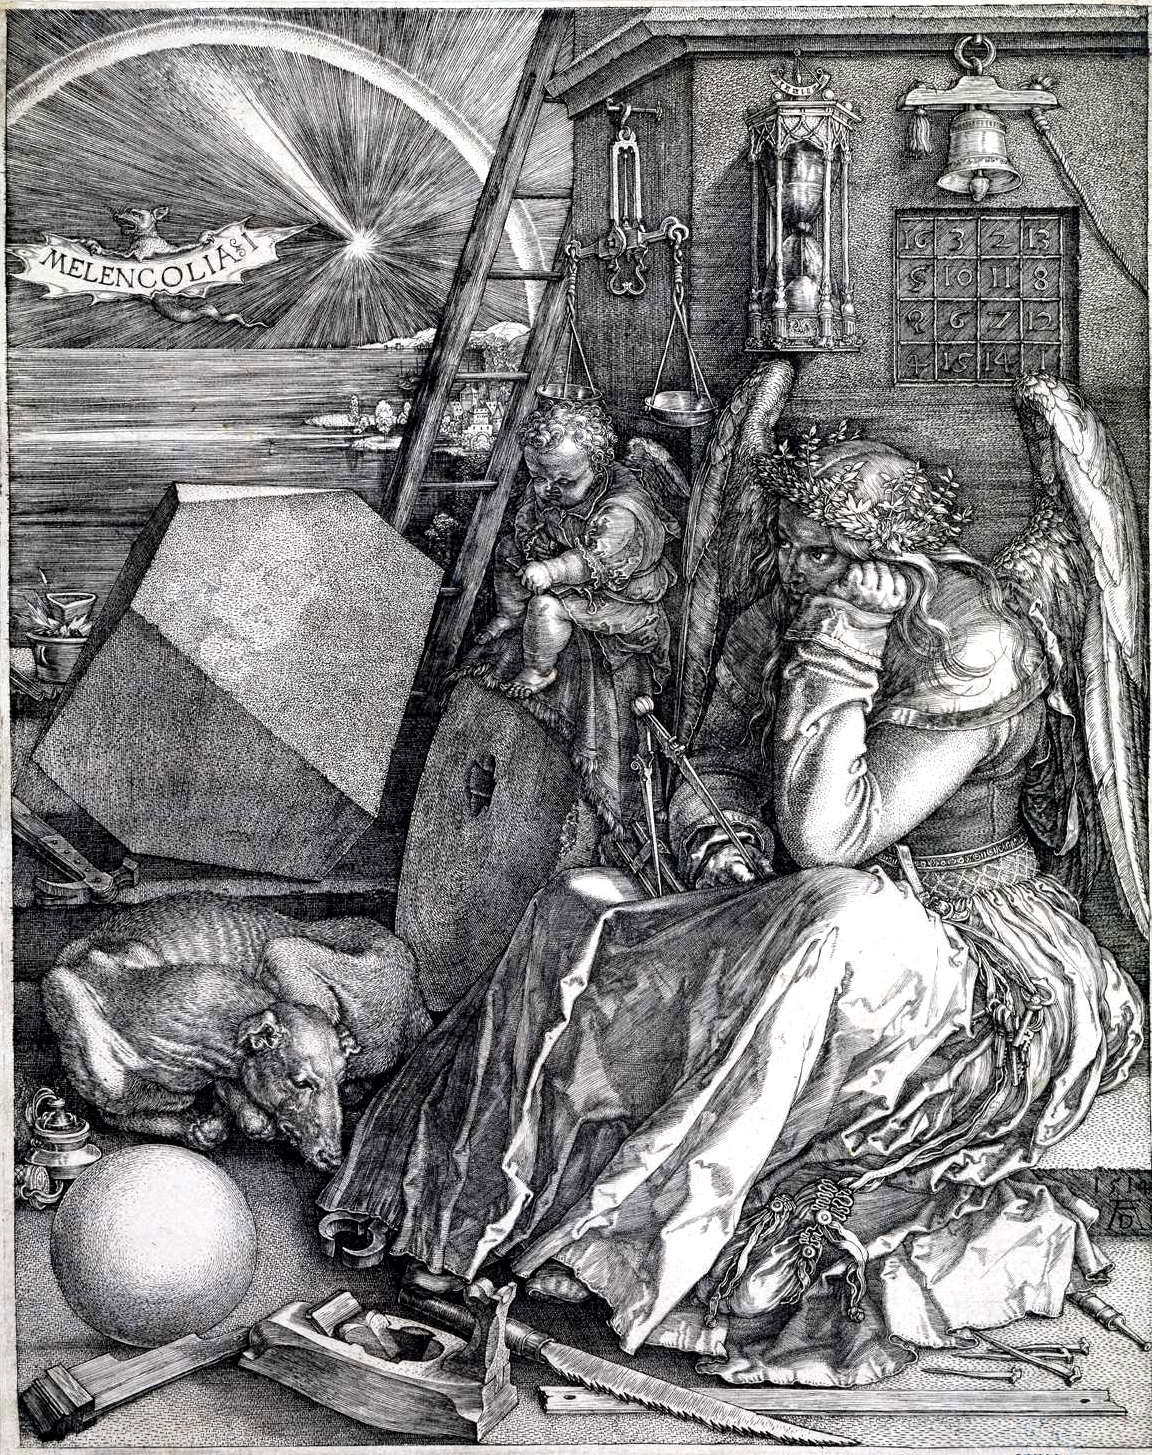
\includegraphics[height=2.5in]{Melencolia.jpg} % wikipedia http://upload.wikimedia.org/wikipedia/commons/1/14/Melencolia_I_%28Durero%29.jpg
\end{center}
One interpretation is that it depicts melancholy, a depressed state.
The figure, genius,
is surrounded by a wealth of fascinating things to be explored.
These include
the compass, the geometrical solid, the scale, and the hourglass.
But the figure is unmoved; all of these things lie unused.
One of the potential delights is the $\nbyn{4}$ matrix in the upper right.
The rows, columns, and diagonals add to $34$.
\begin{center}
  \vcenteredhbox{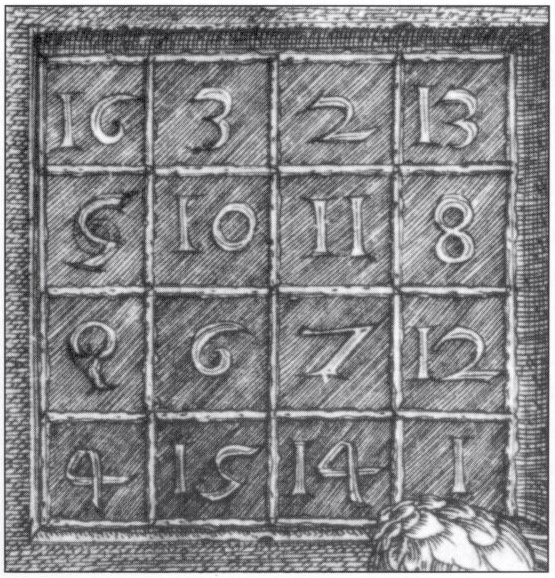
\includegraphics[height=1.25in]{Melencoliadetail.jpg}} % wikipedia http://upload.wikimedia.org/wikipedia/commons/7/7e/Albrecht_D%C3%BCrer_-_Melencolia_I_%28detail%29.jpg
  \qquad
  \begin{tabular}{|c|c|c|c|}
    \hline
      $16$  &$3$  &$2$  &$13$  \\ \hline
      $5$   &$10$ &$11$ &$8$   \\ \hline
      $9$   &$6$  &$7$  &$12$  \\ \hline    
      $4$   &$15$ &$14$ &$1$  \\ \hline    
  \end{tabular}
\end{center}
The middle entries on the bottom row give $1514$, the 
date of the engraving.

A sum of two same-sized magic squares is magic and a 
scalar multiple of a magic square is magic, so the set of 
$\nbyn{n}$ magic squares
$\magicsquares_n$ is a subspace of $\matspace_{\nbyn{n}}$.
The set $\magicsquares_{n,0}$ of $\nbyn{n}$~magic squares with magic number~$0$ 
is another subspace.

A square matrix is \definend{semimagic} if 
the rows and columns add to the same value, that is, we drop the
condition on the diagonals.
The set of semimagic squares $\semimagicsquares_n$ 
is a subspace of $\matspace_{\nbyn{n}}$.
So is the set $\semimagicsquares_{n,0}$  
of $\nbyn{n}$~semimagic squares with magic number~$0$. 

Every $\nbyn{1}$ square is magic, trivially.
If the rows, columns, and diagonals of a $\nbyn{2}$ matrix add to $k$
\begin{equation*}
  \begin{mat}
    a  &b  \\
    c  &d
  \end{mat}
\end{equation*}
then $a+b=s$, $c+d=s$, $a+c=s$, $b+d=s$, $a+d=s$, and $b+c=s$.
\nearbyexercise{exer:TwoByTwoMagicSqUnique} shows that
the system has the unique solution $a=b=c=d=s/2$.
So $\magicsquares_2$ is a one-dimensional subspace of $\matspace_{\nbyn{2}}$.

This Topic shows that for $n>2$ the 
dimension of
$\magicsquares_n$ is $n^2-n$.
We will do this in three steps.

The first step is to show that $\dim\magicsquares_n=\dim\magicsquares_{n,0}+1$.
We define 
the sum of numbers down the upper-left to lower-right diagonal
$\trace (M)=m_{1,1}+\cdots+m_{n,n}$ to be the 
\definend{trace}\index{trace}\index{matrix!trace}
of the matrix~$M$.
We also define
the sum down the other diagonal to be
$\trace^* (M)=m_{1,n}+\cdots+m_{n,1}$.
\nearbyexercise{yy} shows that both of these functions 
$\map{\trace,\trace^*}{\magicsquares_n}{\Re}$ 
are linear.
(We shall use $\trace^*$ in the second step below.)

Observe that 
the nullspace $\nullspace{\trace}$ is the set of magic squares with magic
number zero 
$\magicsquares_{n,0}$.
Observe also that the trace is onto because for any member~$r$ of the 
codomain $\Re$ the $\nbyn{n}$ matrix whose entries are all $r/n$ is
a magic square with magic number~$r$. 

Now recall 
Theorem~Two.II.\ref{th:RankPlusNullEqDim}, that for any linear map the
dimension of the domain equals the dimension of the rangespace 
plus the dimension of the nullspace,
the map's rank plus its nullity.
Here the domain is $\magicsquares_n$, the rangespace is 
$\Re$ and the nullspace is $\magicsquares_{n,0}$,
so we have the $\dim\magicsquares_n=1+\dim\magicsquares_{n,0}$
formula.

The second step of the proof is that 
$\dim\magicsquares_{n,0}=\dim\semimagicsquares_{n,0}+2$.
Consider the function $\map{\theta}{\semimagicsquares_n}{\Re^2}$ that sends a 
matrix~$M$ to
the ordered pair $(\trace(M),\trace^*(M))$.
\nearbyexercise{xx} shows that this function is linear 
and its nullspace is $\magicsquares_{n,0}$,
the $\nbyn{n}$ magic squares with magic number~$0$.

We will show that when $n\geq 3$ the map $\theta$ is onto.
Because $\theta$ is linear we need only find a basis for $\Re^2$ that is the
image of two members of $\mathcal{H}_n$.
Consider the matrix $C\in \mathcal{H}_n$ that has all entries zero except
that the four corners are $c_{1,1}=c_{n,n}=1$ and $c_{1,n}=c_{n,1}=-1$.
Also consider the matrix $D\in \mathcal{H}_n$ with all entries zero except that 
$d_{1,1}=d_{2,2}=1$ and $d_{1,2}=d_{2,1}=-1$.
We have
\begin{equation*}
  \theta(C)=\colvec{2 \\ -2}
  \qquad
  \theta(D)=\begin{cases}
               \binom{2}{-1}  &\text{if $n=3$}  \\[1ex]
               \binom{2}{0}  &\text{if $n>3$}
            \end{cases}
\end{equation*}
and so the image of $\theta$ includes a basis for $\Re^2$ and
thus $\theta$ is onto.

With that, we can again cite that for any linear map the
dimension of the domain equals its rank plus its nullity
to conclude that $\dim(\mathcal{H}_n)=\dim(\magicsquares_{n,0})+2$, as desired.

Our third step is to show that the space 
$\semimagicsquares_{n,0}$ has dimension~$(n-1)^2$.
For that,
let the function $\map{\phi}{\matspace_{\nbyn{n}}}{\matspace_{\nbyn{(n-1)}}}$
be the identity map except that it 
drops the final row and column: $\phi(M)=\hat{M}$ where 
$\hat{m}_{i,j}=m_{i,j}$ for all $i,j\in\setinterval{1}{n-1}$.
The check that $\phi$ is linear is easy.
Consider $\phi$'s restriction to the semimagic squares with 
magic number zero
$\map{\phi}{\semimagicsquares_{n,0}}{\matspace_{\nbyn{(n-1)}}}$.
We claim that this is one-to-one and onto.

To show that it is one-to-one we will show that the only member of 
$\semimagicsquares_{n,0}$ mapped to the zero matrix $Z_{\nbyn{(n-1)}}$
is the zero matrix~$Z_{\nbyn{n}}$.
Suppose that $M\in\semimagicsquares_{\nbyn{n}}$ and $\phi(M)=Z_{\nbyn{(n-1)}}$.
On all but the final row and column $\phi$ is the identity so
the entries in $M$ in all but the final row and column are zero: 
$m_{i,j}=0$ for $i,j\in\setinterval{1}{n-1}$.
The first row of $M$ adds to zero and hence
the final entry in that row $m_{1,n}$ is zero.
Similarly the final entry in each row $i\in\setinterval{1}{n-1}$
and column $j\in\setinterval{1}{n-1}$ is zero.
Then, the final column adds to zero so $m_{n,n}=0$.
Therefore $M$ is the zero matrix $Z_{\nbyn{n}}$ and the restriction of $\phi$ 
is one-to-one. 

To see that the map $\phi$ is onto,
consider a member $\hat{M}$ of the codomain $\matspace_{\nbyn{(n-1)}}$.
We will produce a matrix $M$ from the domain 
$\semimagicsquares_{n,0}$ that maps to it.
The function $\phi$ is the identity on all but the final row and column of 
$M$ so for $i,j\in\setinterval{1}{n-1}$
the entries are $m_{i,j}=\hat{m}_{i,j}$.
\begin{equation*}
  M=\begin{mat}
      \hat{m}_{1,1}    &\hat{m}_{1,2}  &\ldots &\hat{m}_{1,n-1} &m_{1,n}  \\
      \vdotswithin{\hat{m}_{1,1}}  
         &\vdotswithin{\hat{m}_{1,2}}     \\
      \hat{m}_{n-1,1}  &\hat{m}_{n-1,2} &\ldots &\hat{m}_{n-1,n-1} &m_{n-1,n}  \\
      m_{n,1}         &m_{n,2}         &\ldots &m_{n,n-1}        &m_{n,n}  
    \end{mat}
\end{equation*}
The first row of $M$ must add to zero so we take $m_{1,n}$ to be  
$-(\hat{m}_{1,1}+\cdots+\hat{m}_{1,n-1})$.
In the same way we get the final entries 
$m_{i,n}=-(\hat{m}_{i,1}+\cdots+\hat{m}_{i,n-1})$ in all the rows but the 
bottom $i\in\setinterval{1}{n-1}$, 
and the final entries $m_{n,j}=-(\hat{m}_{1,j}+\cdots+\hat{m}_{n-1,j})$ 
in all the columns but the last
$j\in\setinterval{1}{n-1}$.
The entry remaining is the one in the lower right~$m_{n,n}$.
The final column adds to zero so we set it to 
$-(m_{1,n}+\cdots+m_{n-1,n})$ but we must check
that the final row now also adds to zero.
We have $m_{n,n}=-m_{1,n}-\cdots-m_{n-1,n}$ and expanding each of the
$m_{i,n}$ as $-\hat{m}_{1,1}-\cdots-\hat{m}_{1,n-1}$
gives that we have defined $m_{n,n}$ to be the sum of all the entries
of $\hat{M}$.
The sum of the all the entries but the last in the final row is
$m_{1,n}+m_{2,n}+\cdots+m_{n-1,n}$ and expanding each 
$m_{n,j}=-\hat{m}_{1,j}-\cdots-\hat{m}_{n-1,j}$ 
verifies that the sum of the final row is zero.
Thus $M$ is semimagic with magic number zero and so $\phi$ is onto.

Theorem~Two.II.\ref{th:RankPlusNullEqDim} says that for any linear map the
dimension of the domain equals its rank plus its nullity.
Because $\map{\phi}{\semimagicsquares_n}{\matspace_{\nbyn{(n-1)}}}$ is one-to-one
its nullity is zero.
Because it is onto its rank is $\dim(\matspace_{\nbyn{(n-1)}})=(n-1)^2$.
Thus the domain of $\phi$, the subspace  
$\semimagicsquares_{n,0}$ of semimagic squares with magic number zero,
has dimension~$(n-1)^2$.

That finishes the three steps. 
We have that $\dim\magicsquares_n=\dim\magicsquares_{n,0}+1
 =(\dim\semimagicsquares_n-2)+1=(n-1)^2-1=n^2-n$
when $n\geq 3$.


% It is an unsolved problem to determine the number of magic squares of an arbitrary order, but the number of distinct magic squares (excluding those obtained by rotation and reflection) of order n=1, 2, ... are 1, 0, 1, 880, 275305224, ... (Sloane's A006052; Madachy 1979, p. 87). The 880 squares of order four were enumerated by Frénicle de Bessy in 1693, and are illustrated in Berlekamp et al. (1982, pp. 778-783). The number of 5×5 magic squares was computed by R. Schroeppel in 1973. The number of 6×6 squares is not known, but Pinn and Wieczerkowski (1998) estimated it to be (1.7745+/-0.0016)×10^(19) using Monte Carlo simulation and methods from statistical mechanics. 
%(http://mathworld.wolfram.com/MagicSquare.html)


\begin{exercises}
  \item \label{exer:TwoByTwoMagicSqUnique}
    Solve the system $a+b=s$, $c+d=s$, $a+c=s$, $b+d=s$, $a+d=s$, and $b+c=s$.
    \begin{answer}
      For any $k$ we have this.
      \begin{equation*}
        \begin{amat}{4}
          1  &1  &0  &0  &s  \\
          0  &0  &1  &1  &s  \\
          1  &0  &1  &0  &s  \\
          0  &1  &0  &1  &s  \\
          1  &0  &0  &1  &s  \\
          0  &1  &1  &0  &s            
        \end{amat}\;\grstep[-\rho_1+\rho_5]{-\rho_1+\rho_3}\;
        \begin{amat}{4}
          1  &1  &0  &0  &s  \\
          0  &0  &1  &1  &s  \\
          0  &-1 &1  &0  &0  \\
          0  &1  &0  &1  &s  \\
          0  &-1 &0  &1  &0  \\
          0  &1  &1  &0  &s            
        \end{amat}\;\grstep{-\rho_2\leftrightarrow\rho_6}\;
        \begin{amat}{4}
          1  &1  &0  &0  &s  \\
          0  &1  &1  &0  &s  \\          
          0  &-1 &1  &0  &0  \\
          0  &1  &0  &1  &s  \\
          0  &-1 &0  &1  &0  \\
          0  &0  &1  &1  &s  
        \end{amat}\;\grstep[-\rho_2+\rho_4 \\ \rho_2+\rho_5]{-\rho_2+\rho_3}\;
        \begin{amat}{4}
          1  &1  &0  &0  &s  \\
          0  &1  &1  &0  &s  \\          
          0  &0  &2  &0  &s  \\
          0  &1  &-1 &1  &0  \\
          0  &0  &1  &1  &s  \\
          0  &0  &1  &1  &s  
        \end{amat}
      \end{equation*}
      The unique solution is $a=b=c=d=s/2$.
    \end{answer}
  \item Let $M$ be a $\nbyn{3}$ magic square with magic number~$s$.
    \begin{exparts}
      \partsitem Prove that the sum of $M$'s entries is $3s$.
      \partsitem Prove that $s=3\cdot m_{2,2}$.
      \partsitem Prove that $m_{2,2}$ is the average of the entries
        in its row, its column, and in each diagonal.
      \partsitem Prove that $m_{2,2}$ is the median of $M$'s entries.
    \end{exparts}
    \begin{answer}
      \begin{exparts}
        \partsitem The sum of the entries of $M$ is the sum of the sums of
          the three rows. 
        \partsitem The constraints on entries of $M$ involving the center 
          entry make this system.
          \begin{equation*}
            \begin{linsys}{3}
              m_{2,1}  &+  &m_{2,2}  &+  &m_{2,3}  &=  &s  \\ 
              m_{1,2}  &+  &m_{2,2}  &+  &m_{3,2}  &=  &s  \\ 
              m_{1,1}  &+  &m_{2,2}  &+  &m_{3,3}  &=  &s  \\ 
              m_{1,3}  &+  &m_{2,2}  &+  &m_{3,1}  &=  &s  
            \end{linsys}
          \end{equation*}
          Adding those four equations counts each matrix entry once and only
          once, except that the center entry is counted four times.
          Thus the left side sums to $3s+3m_{2,2}$ while the right sums to $4s$.
          So $3m_{2,2}=s$.
        \partsitem
          The second row adds to $s$ so $m_{2,1}+m_{2,2}+m_{2,3}=3m_{2,2}$,
          giving that $(1/2)\cdot(m_{2,1}+m_{2,3})=m_{2,2}$.
          The same goes for the column and the diagonals.
        \partsitem
          By the prior exercise either both $m_{2,1}$ and $m_{2,3}$ are equal
          to $m_{2,2}$ or else one is greater while one is smaller.
          Thus $m_{2,2}$ is the median of the set
          $\set{m_{2,1},m_{2,2},m_{2,3}}$.
          The same reasoning applied to the second column shows that 
          Thus $m_{2,2}$ is the median of the set
          $\set{m_{1,2},m_{2,1},m_{2,2},m_{2,3},m_{3,2}}$.
          Extending to the two diagonals shows it is the median of the set
          of all entries.
      \end{exparts}
    \end{answer}
        

\end{exercises}
\index{magic squares|)}
\endinput


